\documentclass[a4paper]{article}
\usepackage[utf8x]{inputenc}
\usepackage[T1,T2A]{fontenc}
\usepackage[russian]{babel}
\usepackage{hyperref}
\usepackage{indentfirst}
\usepackage{listings}
\usepackage{color}
\usepackage{here}
\usepackage{array}
\usepackage{multirow}
\usepackage{graphicx}
\usepackage{amsmath} 
\usepackage{spverbatim}

\usepackage{caption}
\renewcommand{\lstlistingname}{Программа} % заголовок листингов кода

\lstset{ %
	extendedchars=\true,
	keepspaces=true,
	language=bash,					% choose the language of the code
	basicstyle=\footnotesize,		% the size of the fonts that are used for the code
	numbers=left,					% where to put the line-numbers
	numberstyle=\footnotesize,		% the size of the fonts that are used for the line-numbers
	stepnumber=1,					% the step between two line-numbers. If it is 1 each line will be numbered
	numbersep=5pt,					% how far the line-numbers are from the code
	backgroundcolor=\color{white},	% choose the background color. You must add \usepackage{color}
	showspaces=false				% show spaces adding particular underscores
	showstringspaces=false,			% underline spaces within strings
	showtabs=false,					% show tabs within strings adding particular underscores
	frame=single,           		% adds a frame around the code
	tabsize=2,						% sets default tabsize to 2 spaces
	captionpos=b,					% sets the caption-position to bottom
	breaklines=true,				% sets automatic line breaking
	breakatwhitespace=false,		% sets if automatic breaks should only happen at whitespace
	escapeinside={\%*}{*)},			% if you want to add a comment within your code
	postbreak=\raisebox{0ex}[0ex][0ex]{\ensuremath{\color{red}\hookrightarrow\space}}
}

\usepackage[left=2cm,right=2cm,
top=2cm,bottom=2cm,bindingoffset=0cm]{geometry}
\renewcommand{\labelitemi}{$\diamond$}
\begin{document}	% начало документа

\begin{titlepage}	% начало титульной страницы

	\begin{center}		% выравнивание по центру

		\largeФедеральное государственное автономное образовательное учреждение высшего образования «Санкт-Петербургский политехнический университет Петра Великого» \\
		\large Институт компьютерных наук и технологий \\
		\large Кафедра компьютерных систем и программных технологий\\[2cm]
		% название института, затем отступ 6см
		
	    \vfill
		\hugeТелекоммуникационные технологии\\[0.5cm] % название работы, затем отступ 0,5см
		\large Лабораторная работа №4:\\
		Аналоговая модуляция\\[4.8cm]

	\end{center}

	\begin{flushright} % выравнивание по правому краю
		\begin{minipage}{0.25\textwidth} % врезка в половину ширины текста
			\begin{flushleft} % выровнять её содержимое по левому краю

				\large\textbf{Работу выполнил:}\\
				\large Сергеев ~А.А.\\
				\large {Группа:} 33531/2\\
				
				\large \textbf{Преподаватель:}\\
				\large Богач ~Н.В.\\

			\end{flushleft}
		\end{minipage}
	\end{flushright}
	
	\vfill % заполнить всё доступное ниже пространство

	\begin{center}
	\large Санкт-Петербург\\
	\large \the\year % вывести дату
	\end{center} % закончить выравнивание по центру

\thispagestyle{empty} % не нумеровать страницу
\end{titlepage} % конец титульной страницы
\vfill % заполнить всё доступное ниже пространство

% Содержание
\tableofcontents
\newpage
\section{Цель}
Изучение амплитудной модуляции/демодуляции сигнала.
\section{Постановка задачи}
\begin{enumerate}
    \item Сгенерировать однотональный сигнал низкой частоты.
    \item Выполнить амплитудную модуляцию (АМ) сигнала по закону $$u(t)=(1+MU_m cos(\Omega t))cos(\omega_0 t+\phi_0)$$ для различных значений глубины модуляции М. Использовать встроенную функцию $MatLab ammod$.
    \item Получить спектр модулированного сигнала.
    \item Выполнить модуляцию с подавлением несущей  $$u(t)=MU_m cos(\Omega t))cos(\omega_0 t+\phi_0)$$ Получить спектр.
    \item Выполнить однополосную модуляцию:

$$u(t)=U_m cos(\Omega t)cos(\omega_0 t+\phi_0) + \frac{U_m}{2} \sum_{n=1}^N M_n (cos(\omega_0+\Omega_n)t+\phi_0+\Phi_n)$$
положив $n=1$.
    \item Выполнить синхронное детектирование и получить исходный однополосный сигнал.
    \item Расчитать КПД модуляции. $$\eta_A M = \frac{U_m^2 M^2/4}{P_U} = \frac{M^2}{M^2+1}$$
\end{enumerate}

\section{Теоретический раздел}
Информационные сигналы в основном являются низкочастотными и ограниченными по ширине спектра, в то время как методы передачи сигналов рассчитаны на работу с высокочастотным сигналом. Перенос спектра сигналов из низкочастотной области на заданную частоту, т.е. в выделенную для их передачи область высоких частот выполняется операцией модуляции.\\
$s(t)$ -- низкочастотный сигнал, подлежащий передаче по какому-либо каналу связи. В канале связи для передачи данного сигнала выделяется определенный диапазон высоких частот и формируется вспомогательный периодический высокочастотный сигнал $u(t) = f(t; a_1, a_2, ... a_m).$ Совокупность параметров $a_i$ определяет форму вспомогательного сигнала. Значения параметров $a_i$ в отсутствие модуляции являются величинами постоянными.\\
Если на один из этих параметров перенести сигнал $s(t)$, т.е. сделать его значение пропорционально зависимым от значения $s(t)$ во времени (или по любой другой независимой переменной), то форма сигнала $u(t)$ приобретает новое свойство. Она служит для переноса информации, содержащейся в сигнале $s(t)$. Сигнал $u(t)$ называется несущим сигналом, несущим колебанием или просто несущей, а физический процесс переноса информации на параметры несущего сигнала -- его модуляцией. Исходный информационный сигнал $s(t)$ называют модулирующим, результат модуляции -- модулированным сигналом. Обратную операцию выделения модулирующего сигнала из модулированного колебания называют демодуляцией или детектированием.\\
Наиболее распространенной формой несущих сигналов являются гармонические колебания $u(t)=Ucos(\omega t+\phi)$, которые имеют три свободных параметра: $U$, $\omega$ и $\phi$. В зависимости от того, на какой из данных параметров переносится информация, различают амплитудную (АМ), частотную (ЧМ) или фазовую (ФМ) модуляцию несущего сигнала.\\
При использовании в качестве несущих сигналов периодических последовательностей импульсов (например, прямоугольных) свободными параметрами модуляции могут быть амплитуда, длительность, частота следования и фаза (положение импульса относительно тактовой точки) импульсов. Таким образом, существует три основных вида импульсной модуляции: АИМ, ЧИМ и ФИМ.
\subsection{Амплитудная модуляция (АМ)}
В настоящее время АМ применяется в основном только для радиовещания на сравнительно низких частотах и для передачи изображения в телевизионном вещании. Это вызвано низким КПД использования энергии модулированных сигналов.\\
При АМ выполняется перенос информации $s(t)$ => $U(t)$ при постоянных значениях параметров несущей частоты $\omega$ и $\phi$. АМ – сигнал представляет собой произведение информационной огибающей $U(t)$ и гармонического колебания ее заполнения с более высокими частотами: $$U(t)=U_m[1+Ms(t)],$$ где $U_m$ - постоянная амплитуда несущего колебания при отсутсвии входного (модулирующего) сигнала $s(t)$, $M$ -- глубина АМ.\\
Если модулирующий сигнал представлен одночастотным гармоническим колебанием с амплитудой $S_0$, то коэффициент модуляции равен отношению амплитуд модулирующего и несущего колебания $M=S_0/U_m$. Значение М должно находиться в пределах от $0$ до $1$ для всех гармоник модулирующего сигнала. При значении М<1 форма огибающей несущего колебания полностью повторяет форму модулирующего сигнала $s(t)$.\\
Простейшая форма модулированного сигнала создается при однотональной амплитудной модуляции -- модуляции несущего сигнала гармоническим колебанием с одной частотой $\Omega$: $$u(t)=U_m[1+Mcos(\Omega t)]cos(\omega_0 t)$$
Основная теорема модуляции:$$u(t)=U_m cos(\omega_0 t) + \frac{U_m M}{2} cos[(\omega_0 + \Omega)t] + \frac{U_m M}{2} cos[(\omega_0 - \Omega)t].$$
Модулирующее колебание с частотой $\Omega$ перемещается в область частоты $\omega_0$ и расщепляется на два колебания, симметричные относительно частоты $\omega_0$, с частотами соответственно $(omega_0 + \Omega)$ - верхняя боковая частота, и $(omega_0 - \Omega)$ - нижняя боковая частота. Физическая ширина спектра модулированного сигнала в два раза больше ширины спектра сигнала модуляции.\\
КПД АМ: $$\eta_{AM}=\frac{U_m^2 M^2 /4}{P_U} = \frac{M^2}{M^2+2}.$$
Отсюда следует, что при $M=1$ КПД амплитудной модуляции составляет только $33$, а на практике обычно меньше $20$.\\
При идентичности информации в группах верхних и нижних боковых частот нет необходимости в их одновременной передаче. Одна из них перед подачей сигнала в канал связи может быть удалена, чем достигается двукратное сокращение полосы занимаемых сигналом частот.\\
Для верхней или нижней боковой полосы:
$$u(t)=U_m cos(\Omega t)cos(\omega_0 t+\phi_0) + \frac{U_m}{2} \sum_{n=1}^N M_n (cos(\omega_0 \pm \Omega_n)t \pm \phi_0 \pm \Phi_n)$$
Внешняя форма ОБП-сигнала сходна с обычным АМ-сигналом, но ее огибающая имеет в два раза меньшую амплитуду по сравнению с АМ при $M = 1$.
\subsection{Синхронное детектирование}
При синхронном детектировании модулированный сигнал умножается на опорное колебание с частотой несущего колебания. Без учета начальных фаз колебаний: $$y(t)=u(t)cos \omega_0 t cos \omega_0 t = \frac{1}{2}U(t)+\frac{1}/{2} U(t) cos 2 \omega_0 t.$$
сигнал разделяется на два слагаемых, первое из которых повторяет исходный модулирующий сигнал, а второе повторяет модулированный сигнал на удвоенной несущей частоте $2 \omega_0$. Форма новой несущей при синхронном детектировании является чистой гармоникой, в отличие от двухполупериодного детектирования, где новая несущая содержит дополнительные гармоники более высоких частот. Физический амплитудный спектр сигналов после демодуляции подобен спектру двухполупериодного детектирования, но однозначно соотносится со спектром входного модулированного сигнала: амплитуды гармоник модулированного сигнала на частоте $2 \omega_0$ в два раза меньше амплитуд входного сигнала, постоянная составляющая равна амплитуде несущей частоты $\omega_0$ и не зависит от глубины модуляции, амплитуда информационного демодулированного сигнала в два раза меньше амплитуды исходного модулирующего сигнала. Особенностью синхронного детектирования является независимость от глубины модуляции, т.е. коэффициент модуляции сигнала может быть больше единицы.
\section{Ход работы}
\subsection{Генерация сигнала}
\lstinputlisting[language=Matlab]{lab4/sig.m}\\
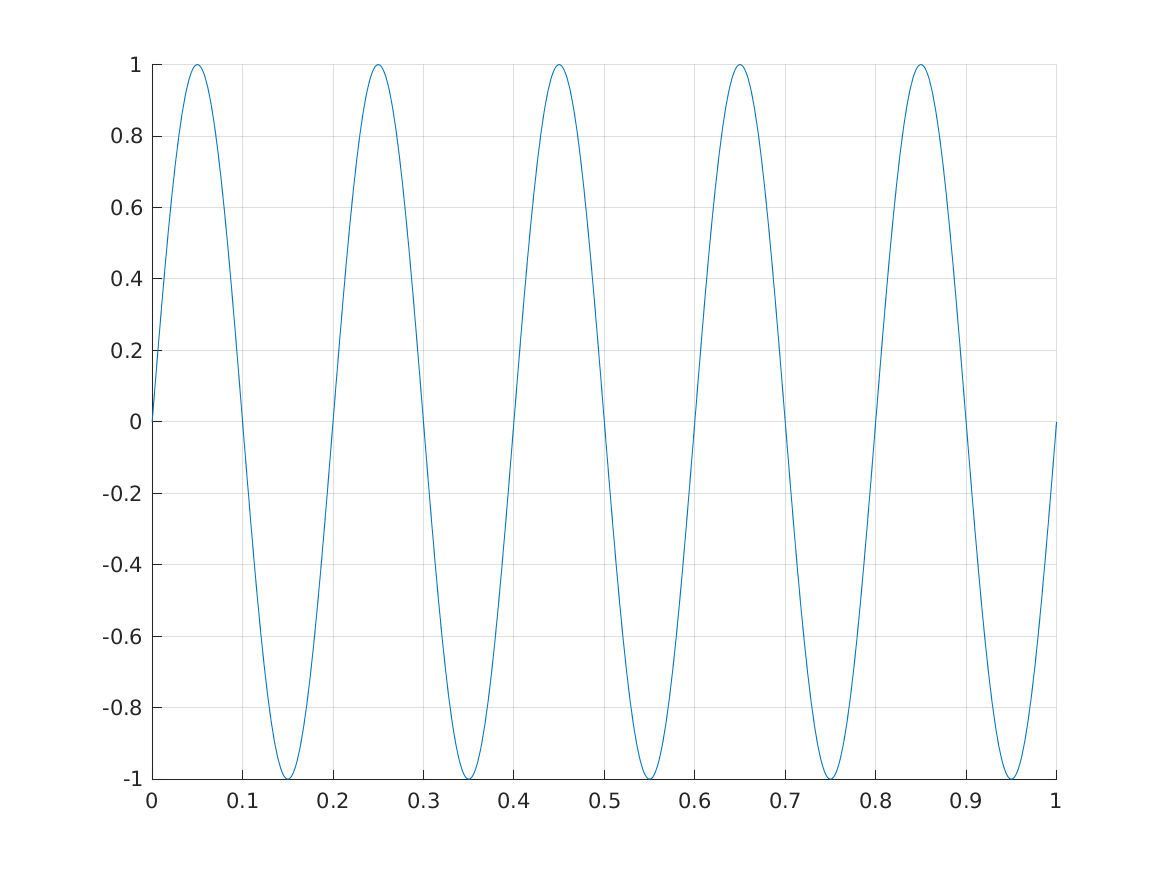
\includegraphics[scale=0.7]{lab4/figures/figure_0.png}\\
\subsection{Амплитудная модуляция}
\lstinputlisting[language=Matlab]{lab4/amplitude_modulation.m}\\
\subsubsection{Амплитудная модуляция при M = 1}
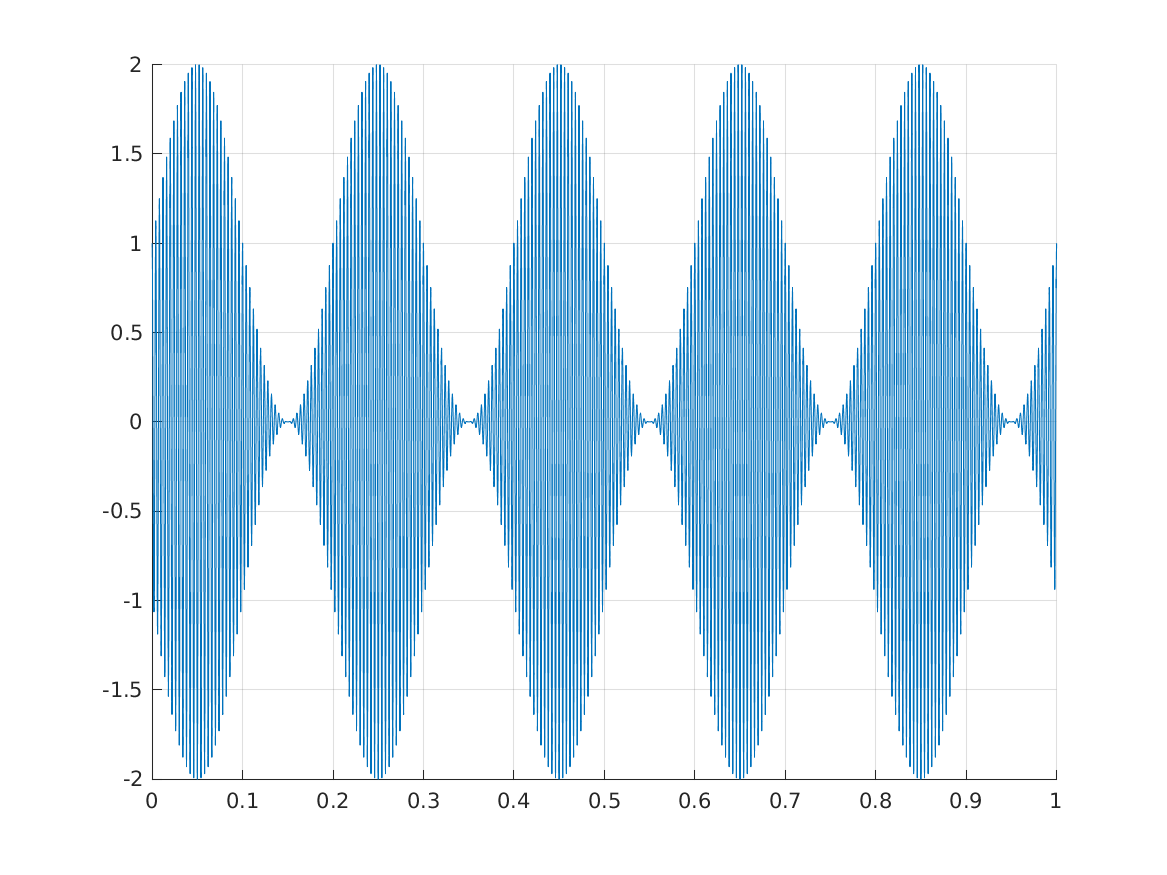
\includegraphics[scale=0.45]{lab4/figures/figure_1.png}
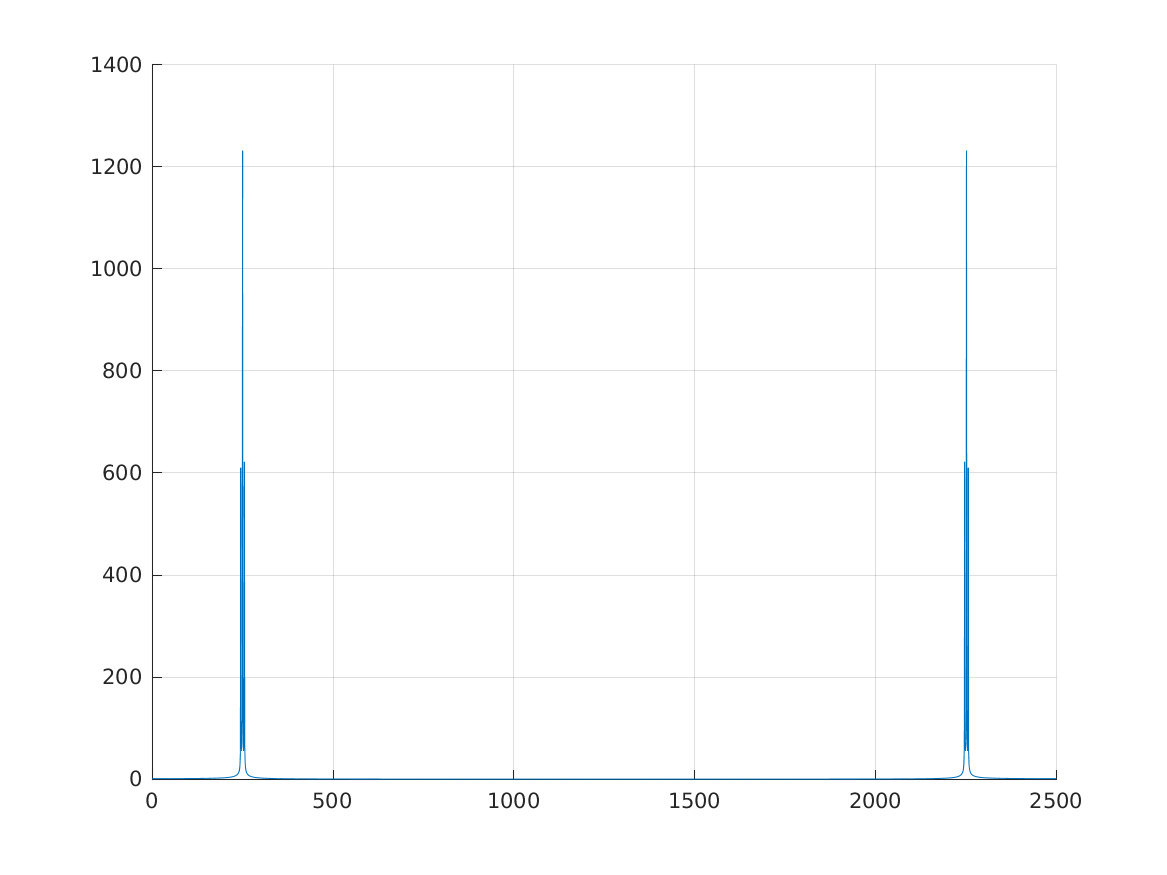
\includegraphics[scale=0.45]{lab4/figures/figure_2.png}\\
\subsubsection{Амплитудная модуляция при M = 2}
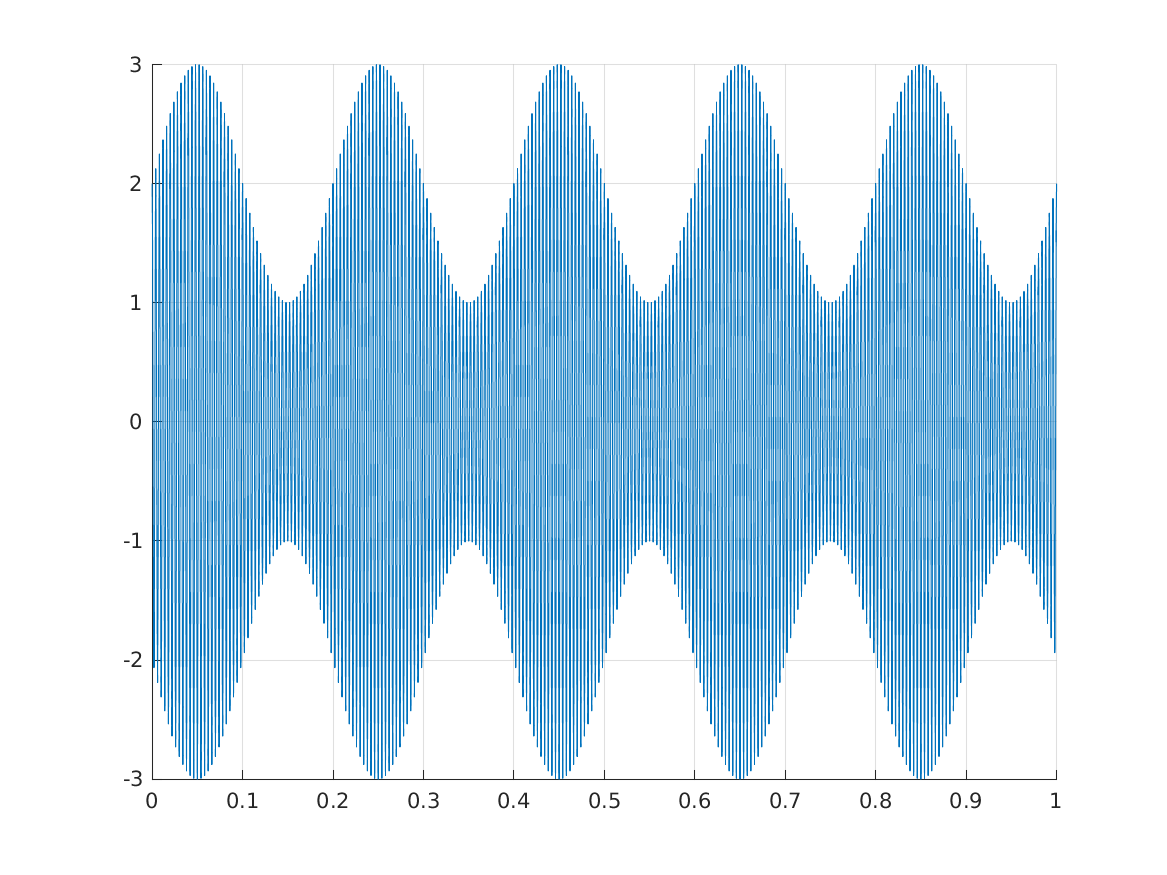
\includegraphics[scale=0.45]{lab4/figures/figure_3.png}
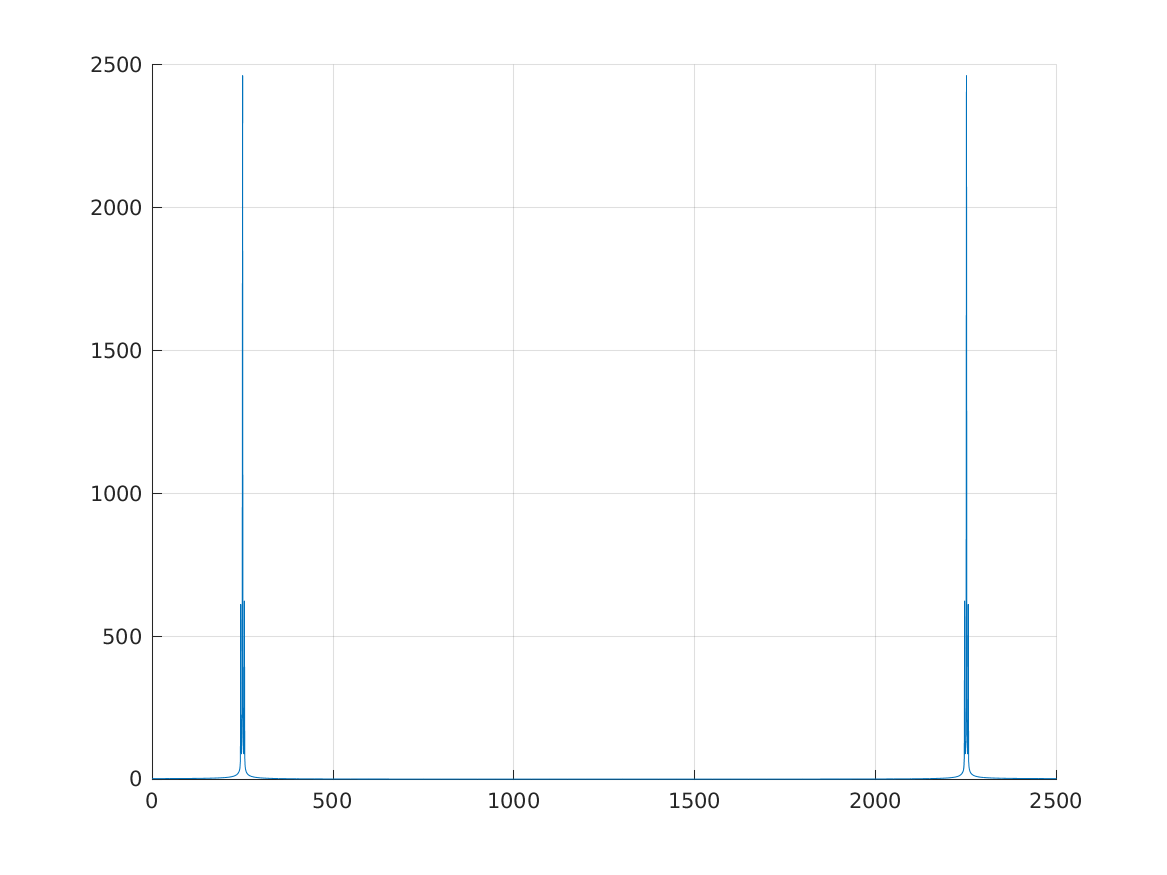
\includegraphics[scale=0.45]{lab4/figures/figure_4.png}\\
\subsection{Модуляция с подавлением несущей}
\lstinputlisting[language=Matlab]{lab4/amplitude_modulation_with_carrier_suppression.m}\\
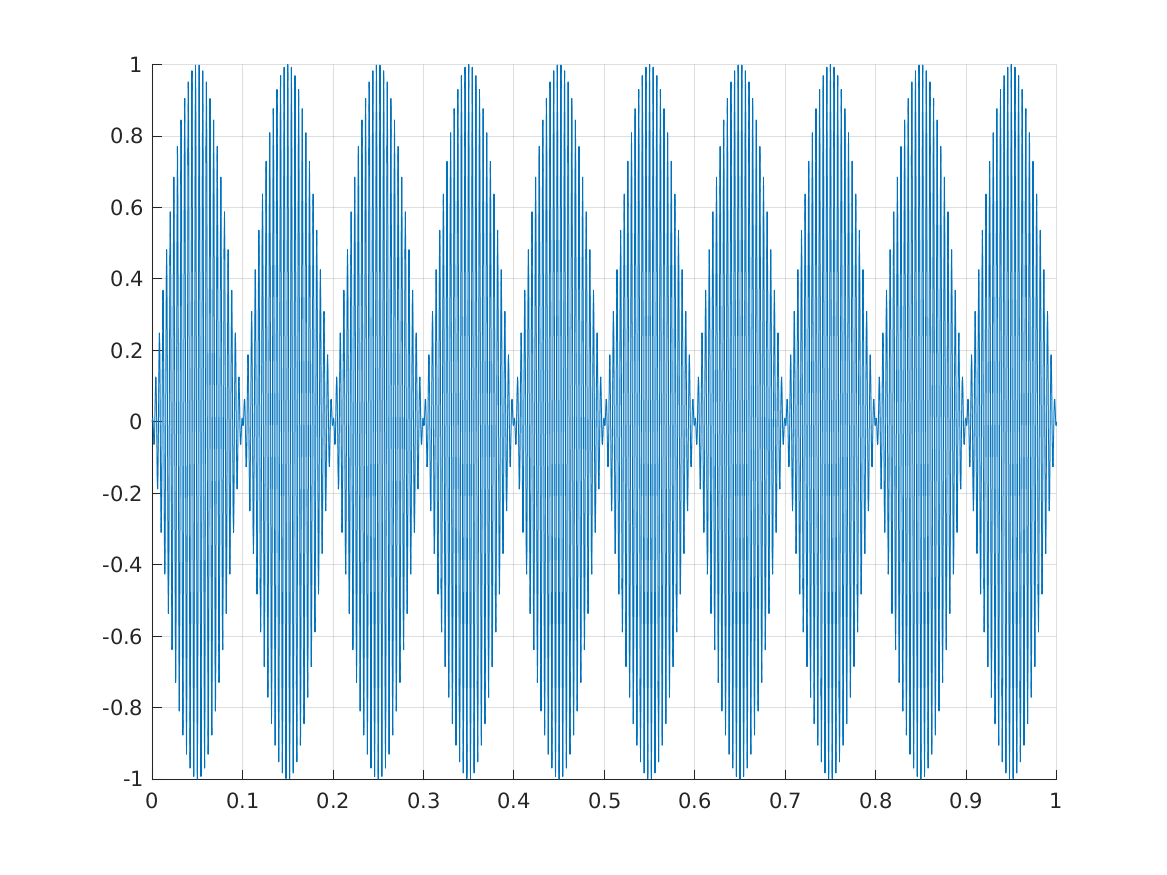
\includegraphics[scale=0.45]{lab4/figures/figure_5.png}
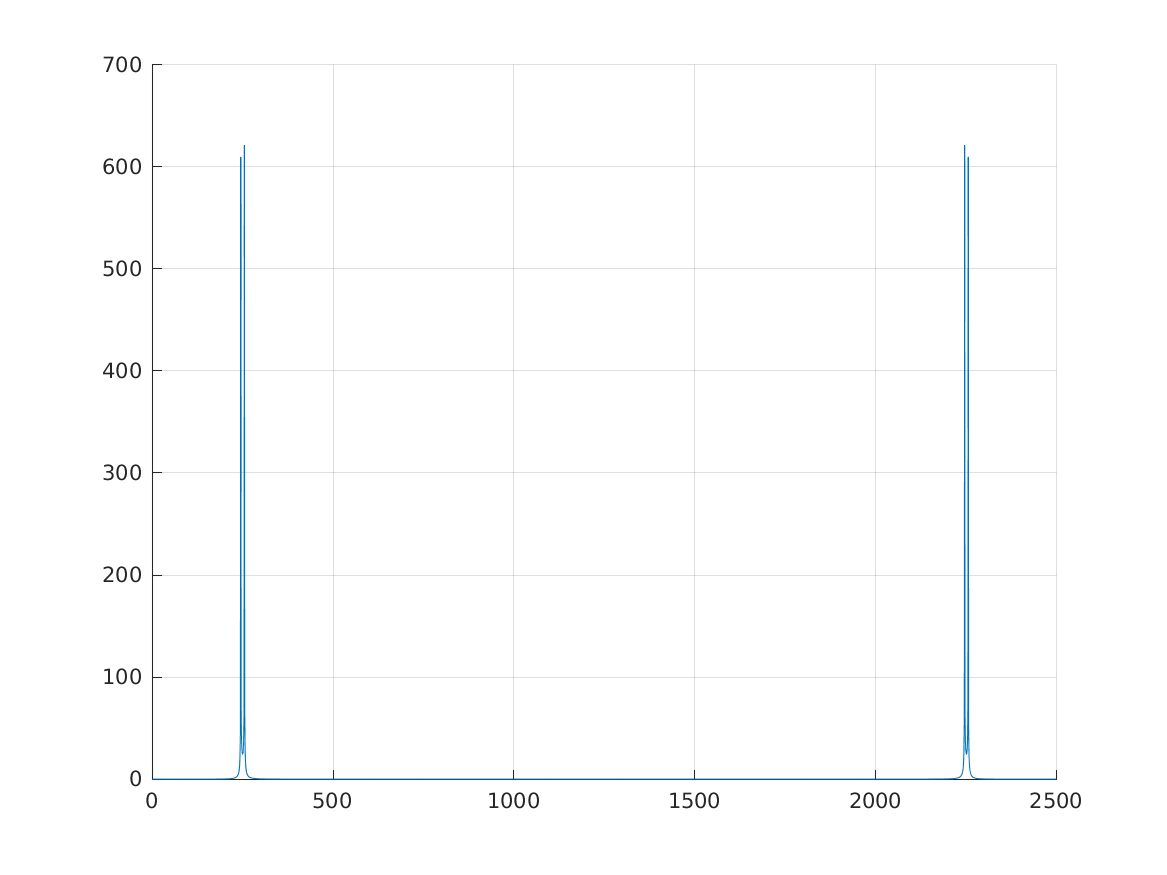
\includegraphics[scale=0.45]{lab4/figures/figure_6.png}\\
\subsection{Однополосная модуляция и детектирование сигнала}
\lstinputlisting[language=Matlab]{lab4/single_band_modulation_and_signal_detection.m}\\
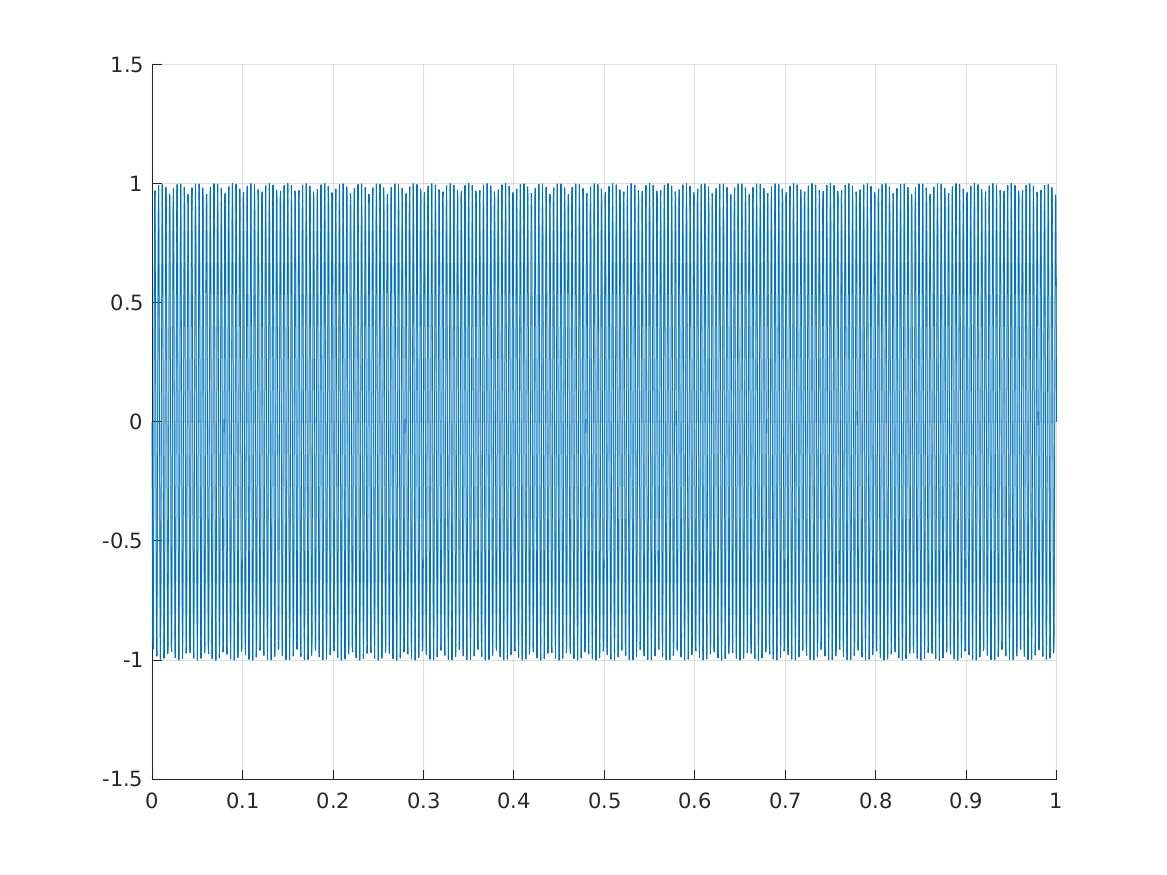
\includegraphics[scale=0.45]{lab4/figures/figure_7.png}
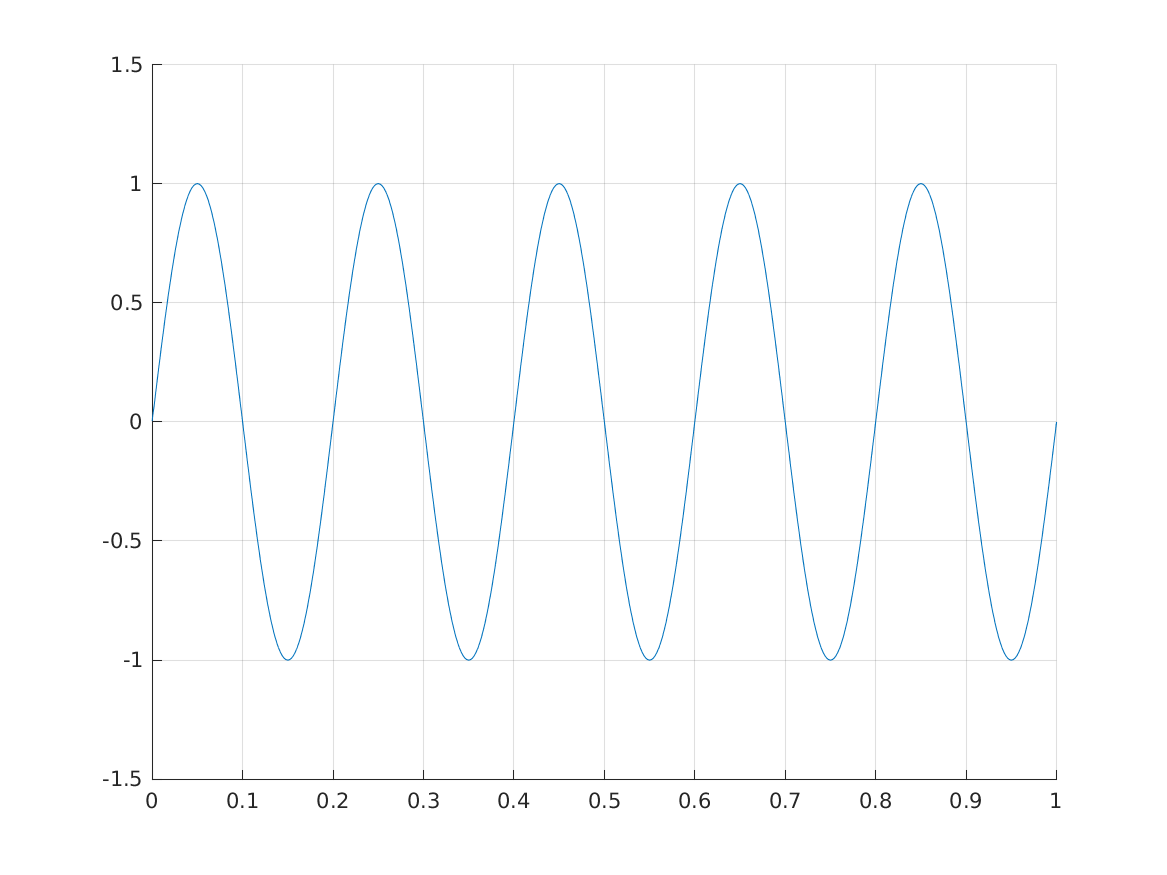
\includegraphics[scale=0.45]{lab4/figures/figure_8.png}\\
Как мы видим, демодулированный сигнал совпал с исходным\\
\section{Вывод}
 Основными достоинствами амплитудной модуляции является узкая ширина спектра АМ сигнала, а также простота получения модулированных сигналов.\\
К недостаткам можно отнести низкую помехоустойчивость (т. к. при воздействии помехи на сигнал искажается его форма -- огибающая, которая и содержит передаваемое сообщение) и неэффективное использование мощности передатчика.\\
Амплитудная модуляция нашла широкое применение в системах телевизионного вещания (для передачи телевизионных сигналов), в системах звукового радиовещания и радиосвязи на длинных и средних волнах.
\end{document}